\section{Materials \& Methods}
\subsection{Participants \& Ethical Standards \textcolor{green}{Sezen, Lukas}}
We recruited 20 participants (\todo{gender and age of participants} female), all right-handed. No participant had experienced VR with vibrotactile feedback. Participants received 10 Euro per hour as compensation for their participation. The study design was approved by the local ethics committee and all participants provided written informed consent prior to their participation. 

\subsection{Procedure \& Data acquisition \textcolor{green}{Sezen, Lukas}}
The apparatus and general procedure are explained in detail elsewhere \citep{Gehrke_2019}. Here, we focus on the description of EEG data processing using more trials and participants with respect to the previous report. Compared to \citep{Gehrke_2019} we focus solely on two feedback conditions, visual only (V) as well as visual together with vibration at the fingertip (VT). Due to the interest in processing mismatches, we run linear regression analyses only on those trials.

%EEG and mocap here: how was it extended over gehrke paper?

\begin{figure}
    \centering
    \includegraphics[width=\textwidth]{figures/pe_task.pdf}
    \caption{Caption}
    \label{fig:my_label}
\end{figure}

\begin{comment}
\begin{figure}[h]
  \centering
  \begin{minipage}[]{\textwidth}
    \begin{flushleft}\textbf{A}\end{flushleft}
    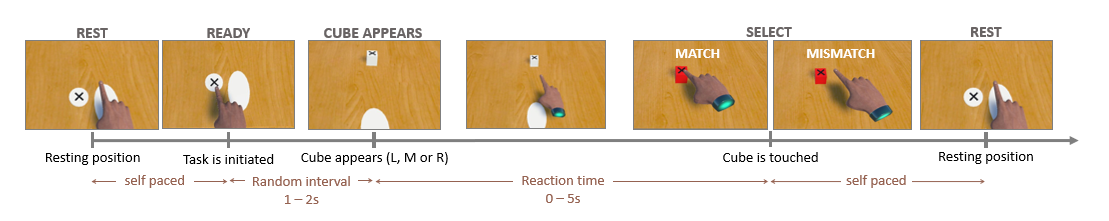
\includegraphics[width=\textwidth]{figures/Task_mismatch.PNG}
    \label{histR}
  \end{minipage}
  
  \begin{minipage}[]{0.33\textwidth}
    \begin{flushleft}\textbf{B}\end{flushleft}
    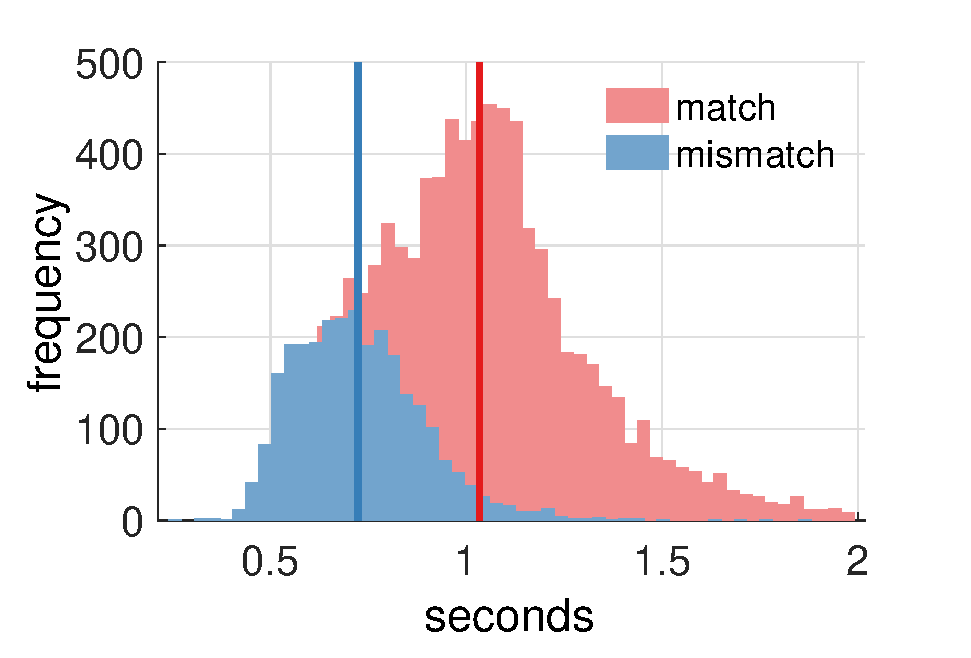
\includegraphics[width=\textwidth]{figures/histRT.eps}
    \label{histR}
  \end{minipage}
  \begin{minipage}[]{0.33\textwidth}
    \begin{flushleft}\textbf{C}\end{flushleft}
    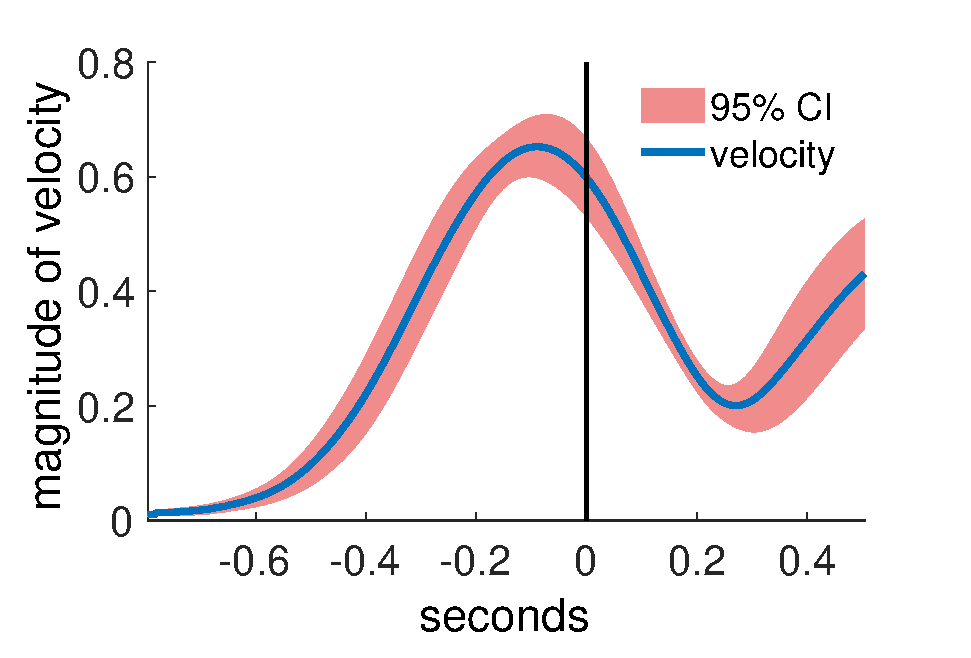
\includegraphics[width=\textwidth]{figures/vel_profile.eps}
    \label{histR}
  \end{minipage}
  \begin{minipage}[]{0.33\textwidth}
    \begin{flushleft}\textbf{D}\end{flushleft}
    \includegraphics[width=\textwidth]{figures/erpimage2D_vel.eps}
    \label{histR}
  \end{minipage}
  \caption{A, B, C, D, E}
\end{figure}
\end{comment}


% brief summary over the following methods section:
% - mass univariate regression at the single subject level (Kutas rERP, Groppe, Pernet, Cavanagh, Cohen). Averaging betas and pvals, then do tfce transform on the mean and infer on the tfce statistic? \todo{check if this method correct, how did cohen do it?}
% - \subsubsection{Group level inference and its multiple comparison correction}
% - paired ttest with bootstrap-tfce multiple comparison correction \citep{SMITH200983} to make inferences about the interaction
